\documentclass[12pt,titlepage]{article}

\usepackage{amsmath,amsthm}
\usepackage{unicode-math}
\usepackage{xltxtra}
\usepackage{xgreek}

\setmainfont{Times New Roman}

\usepackage{tikz}
\pagestyle{empty}

\usepackage{geometry}
 \geometry{a4paper, top=10mm, bottom=10mm, left=10mm, top=10mm}
 \begin{document}

 \section*{Δευτεροβάθμιες εξισώσεις}

   Ένας εύκολος τρόπος να λυθεί μία εξίσωση $$αx^2+βx+γ=0\text{, }α\ne 0$$ είναι να υπολογίσουμε την διακρίνουσα $Δ=β^2-4αγ$. Αν

 \begin{itemize}
   \item $Δ>0$ η εξίσωση έχει δύο πραγματικές ρίζες στο $\mathbb{R}$ τις $x_{1,2}=\frac{-β\pm \sqrt{Δ}}{2α}$
   \item $Δ=0$ η εξίσωση έχει μία διπλή πραγματική ρίζα την $x=-\frac{β}{2α}$
   \item $Δ< 0$ η εξίσωση έχει δύο μιγαδικές ρίζες τις $z_{1,2}=\frac{-β\pm i\sqrt{-Δ}}{2α}$
 \end{itemize}

\subsection*{Γραφική παράσταση}
 Η γραφική παράσταση της συνάρτησης $f(x)=x^2-1$ είναι η

 \begin{figure}[h]
   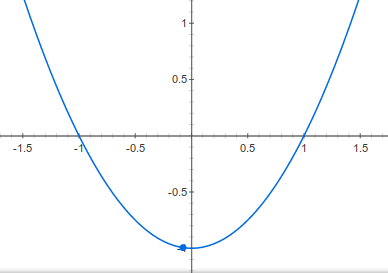
\includegraphics[width=0.4\textwidth]{plot.png}
 \end{figure}

 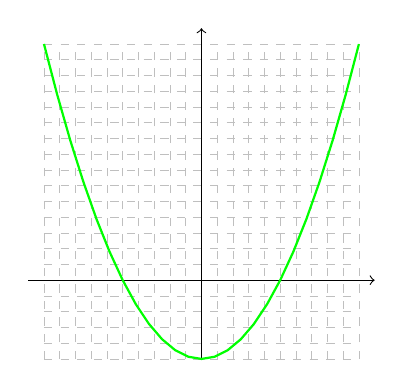
\begin{tikzpicture}
  \draw [help lines,color=gray!50, dashed, step=0.2] (-2,-1) grid (2,3);
  \draw [->] (-2.2,0) -- (2.2,0);
  \draw [->] (0,-1) -- (0,3.2);
  \draw [green, thick, domain=-2:2] plot (\x, {\x*\x-1});
 \end{tikzpicture}


 \def\iangle{35} % Angle of the inclined plane
 \def\down{-90}
 \def\arcr{0.5cm} % Radius of the arc used to indicate angles


 \begin{tikzpicture}[
    force/.style={>=latex,draw=blue,fill=blue},
    axis/.style={densely dashed,gray,font=\small},
    M/.style={rectangle,draw,fill=lightgray,minimum size=0.5cm,thin},
    m/.style={rectangle,draw=black,fill=lightgray,minimum size=0.3cm,thin},
    plane/.style={draw=black,fill=blue!10},
    string/.style={draw=red, thick},
    pulley/.style={thick},
]

\matrix[column sep=1cm] {
    %% Sketch
    \draw[plane] (0,-1) coordinate (base)
                     -- coordinate[pos=0.5] (mid) ++(\iangle:3) coordinate (top)
                     |- (base) -- cycle;
    \path (mid) node[M,rotate=\iangle,yshift=0.25cm] (M) {};
    \draw[pulley] (top) -- ++(\iangle:0.25) circle (0.25cm)
                   ++ (90-\iangle:0.5) coordinate (pulley);
    \draw[string] (M.east) -- ++(\iangle:1.5cm) arc (90+\iangle:0:0.25)
                  -- ++(0,-1) node[m] {};

    \draw[->] (base)++(\arcr,0) arc (0:\iangle:\arcr);
    \path (base)++(\iangle*0.5:\arcr+5pt) node {$\alpha$};
    %%

&
    %% Free body diagram of M
    \begin{scope}[rotate=\iangle]
        \node[M,transform shape] (M) {};
        % Draw axes and help lines

        {[axis,->]
            \draw (0,-1) -- (0,2) node[right] {$+y$};
            \draw (M) -- ++(2,0) node[right] {$+x$};
            % Indicate angle. The code is a bit awkward.

            \draw[solid,shorten >=0.5pt] (\down-\iangle:\arcr)
                arc(\down-\iangle:\down:\arcr);
            \node at (\down-0.5*\iangle:1.3*\arcr) {$\alpha$};
        }

        % Forces
        {[force,->]
            % Assuming that Mg = 1. The normal force will therefore be cos(alpha)
            \draw (M.center) -- ++(0,{cos(\iangle)}) node[above right] {$N$};
            \draw (M.west) -- ++(-1,0) node[left] {$f_R$};
            \draw (M.east) -- ++(1,0) node[above] {$T$};
        }

    \end{scope}
    % Draw gravity force. The code is put outside the rotated
    % scope for simplicity. No need to do any angle calculations.
    \draw[force,->] (M.center) -- ++(0,-1) node[below] {$Mg$};
    %%

&
    %%%
    % Free body diagram of m
    \node[m] (m) {};
    \draw[axis,->] (m) -- ++(0,-2) node[left] {$+$};
    {[force,->]
        \draw (m.north) -- ++(0,1) node[above] {$T'$};
        \draw (m.south) -- ++(0,-1) node[right] {$mg$};
    }

\\
};
\end{tikzpicture}

 \end{document}
